 
 %~\cite[p. 2]{evans2008social} -> example
 
 \chapter{Background}
 \label{sec:background}
 
 
 This chapter explains the theoretical background used for the development of an entity based sentiment classifier. The chapter is divided into three sections: \autoref{sec:socialMedia} explains the basic concepts related to the social media and the social networking service Twitter. In \autoref{sec:sentAnalysis} Sentiment Analysis is defined and different state-of-the-art sentiment classification techniques are described. Finally, \autoref{sec:ner} explores existing Named Entity Recognition approaches.
 
 \section{Social Media}
 \label{sec:socialMedia}
 
Social Media refers to a set of computer-based tools that allows people, organizations and companies to share and exchange information with community networks. Moreover, Social Media tends to change with time allowing people to create content in a dynamic way and without restrictions. Therefore, there is an unquantifiable number of communities performing all kinds of activities such as blogging, posting on forums, podcasting, generating trends on social networks and more. 

The Social Media relies on various technologies to achieve a compelling communication between users. Web structures like social networks are fundamental for the social media. These structures are mainly made of actors and messages which can be visualized as graph nodes with specific properties and unique attributes. This concept is depicted on \autoref{fig2:twitter_graph} where the interaction between the different elements of the social network Twitter is represented. In \autoref{sec:twitter}, Twitter and its elements are explained in detail.

\begin{figure}
    \centering
    \caption[Twitter graph representation]{Twitter: graph representation {~\cite{kenny2014graph}}}
    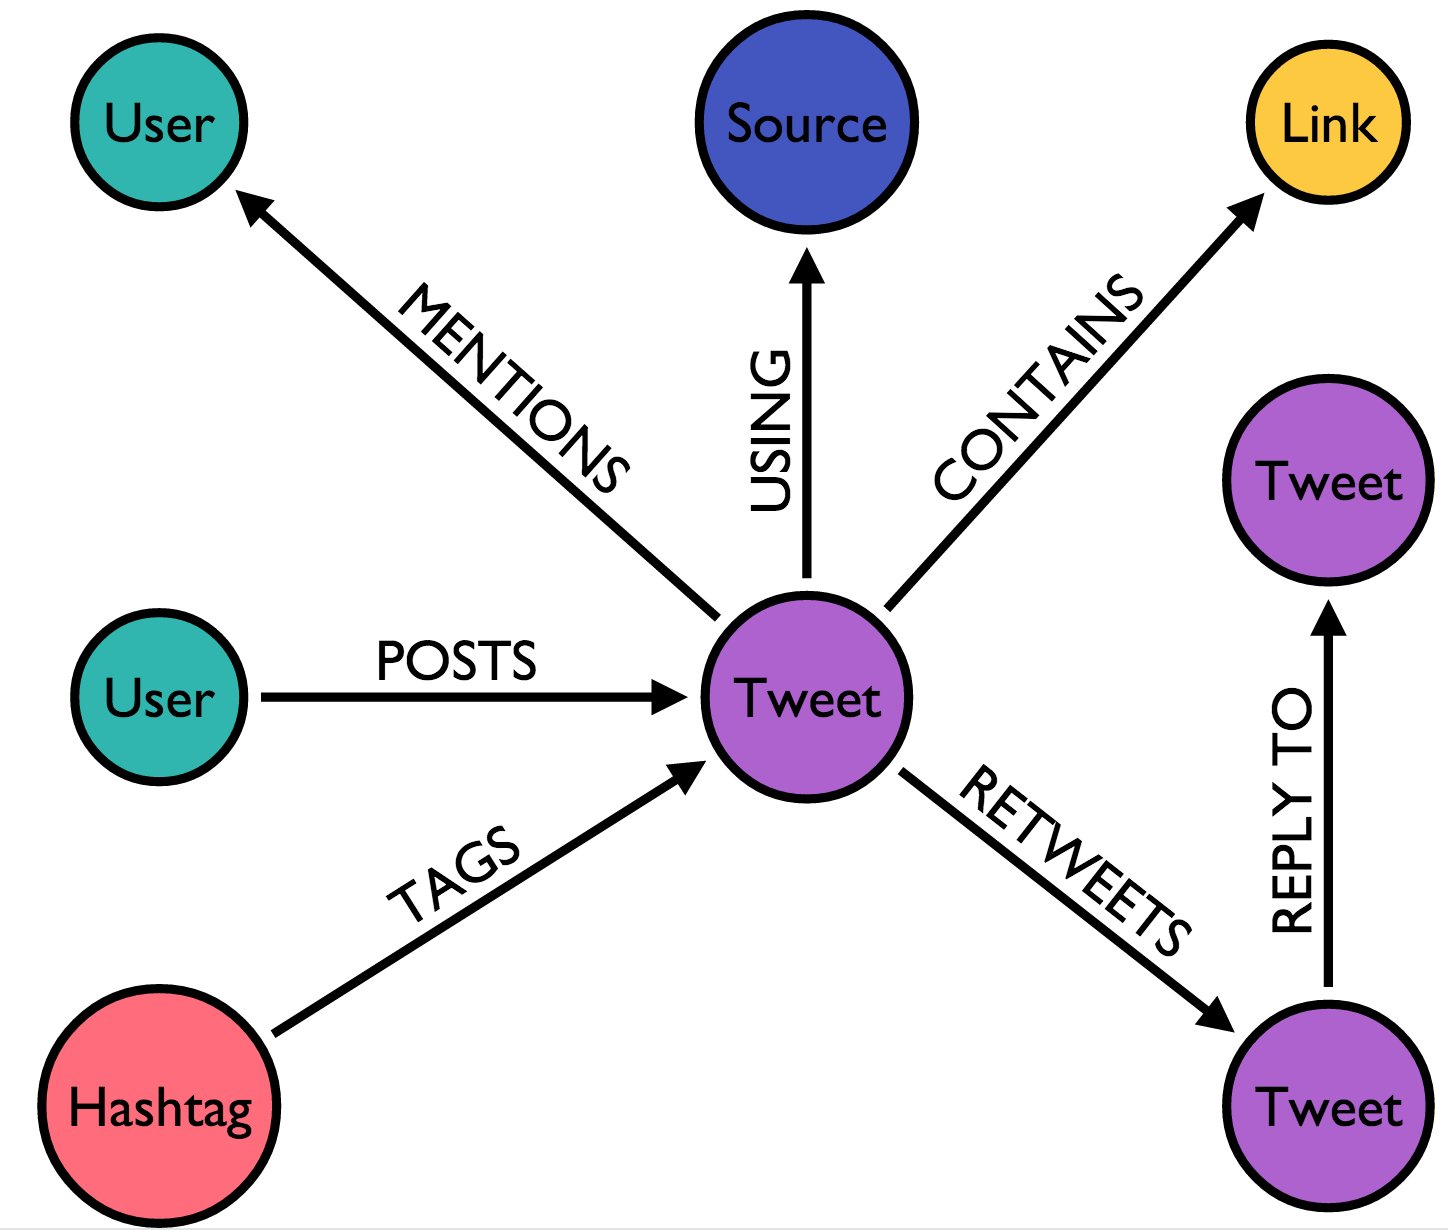
\includegraphics[width=\linewidth]{02_twitter_graph.png}
    \label{fig2:twitter_graph}
\end{figure}

\subsection{Twitter}
\label{sec:twitter}

Being one of the most popular websites in the world, Twitter has become an ever-growing corpus of information. As a social network, Twitter allows constant sharing of short messages between users; this is also called micro-blogging. Between users, they can follow the activity of each other giving updates of their messages. Currently, this network has around 320 million of active users {~\cite{statTwit2016}.

As described in \autoref{fig2:twitter_graph}, Twitter is composed of the following elements:

\begin{itemize}
\item \textbf{Tweet:} Tweets are the essence of Twitter, they are short message units (pieces of information) formed by a maximum of 140 characters. Users use tweets to share ideas, status, news or any other kind of information with their followers. In \autoref{fig3:tweet_example} a tweet example is showed where the actor: User is \textit{"Outlook"} and the message contains \textit{\#hashtags, @mentions} and \textit{URLs}. 

\pagebreak

\begin{figure}
    \centering
    \caption{A tweet example}
    
\includegraphics[width=\linewidth]{03_tweet_example.png}
    \label{fig3:tweet_example}
\end{figure} 

\item \textbf{Users:} The users are the source of information on Twitter. They have followers who are other users interested in the content being sharing.
\item \textbf{Trends:} Trends are popular topics close to the geographic location of the users. They are determined by an algorithm that combines the information about followers, accounts, and places related to them. The trends intend to help users to discover relevant topics based on their location.  
\end{itemize}

\section{Sentiment Analysis}
\label{sec:sentAnalysis} 
 
 Sentiment analysis (SA) also known as Opinion Mining can be defined as the use of computer-based methods to extract an opinion from a given text source. Liu ~\cite[p. 7]{liu2012sentiment} defines SA as: 
 \begin{displayquote}
"The field of study that 
analyzes people’s opinions, sentiments, evaluations, appraisals, attitudes, 
and emotions towards entities such as products, services, organizations, 
individuals, issues, events, topics, and 
their attributes."
\end{displayquote}
    
Opinions are essential for all human activities because they affect our decisions. Before making decisions, people usually evaluate others opinions. In the real world, businesses and organizations are always trying to know the public opinion about their
products and services and be able adapt marketing strategies~\cite[p. 10]{liu2012sentiment}. Nowadays, companies may no longer require surveys and opinion polls to gather the opinion of their customers. However, analyzing opinion sites and social networks by SA means is not an easy task. Several fields of Computer Science such as Natural Language Processing (NLP), Machine Learning (ML) and Information Retrieval (IR) are some of the research areas involved in SA. 

\subsection{Analysis Levels}

There are different levels of SA that could be applied to a given text source, these are the following~\cite[p. 11]{liu2012sentiment}:
 
\begin{itemize}

\item \textbf{Document level:} The objective of this level if SA is to classify the sentiment (positive, negative or neutral) of a whole document. Documents in this context refer to any piece of information that requires analysis. Tweets, .pdf files, forums posts, e-commerce reviews, all are considered documents for sentiment analysis porpoises. Sentiment classification of product reviews on e-commerce system are good examples of these level of analysis. Document level SA is effective on text sources that express opinion towards a single entity. When many entities are present in the document this type of analysis may not be very accurate.

\item \textbf{Sentence level:} As its name describes, sentence level analysis segments a given document into sentences, then each of these sentences is processed for classification. Similar to \textit{document-level} SA, opinions on sentences must express its sentiment towards a single entity in order to achieve high accuracy. 

\item \textbf{Entity level:} \textit{document-level} and \textit{sentence-level} analysis are not capable of finding the target of peoples’ opinion. Entity-level is a finer-grained analysis that assumes the presence of a target entity in the opinion expression. For example, the sentence \textit{"although the iPhone is not a good phone, I still love Apple as a company"} may appear to have a positive tone but is not accurate to classify it as positive. In this case, there are two different sentiments: A positive sentiment towards the entity \textit{Apple} and a negative sentiment towards entity \textit{iPhone}. Therefore, the ultimate goal of this level of analysis is to find out the sentiment expressed towards target entities. This thesis project base its’ sentiment classification approach on this level of analysis.

\end{itemize}

\subsection{Sentiment Classification}
\label{sec:sentClassification} 

Sentiment classification is one of the most studied topics in the area of sentiment analysis and natural language processing. The main goal is to classify a document as positive or negative based on the opinion expressed in it, if the document does not contain any opinion expression the classification result must be neutral. The following sections present unsupervised and supervised techniques for sentiment classification according to Bing Liu~\cite{liu2012sentiment}.

 

 
 \subsubsection{Unsupervised Techniques}
 
 Unsupervised techniques for sentiment classification are strongly based on opinion words, also known as lexical resources. Consequently, these techniques classify documents using lexicon-based methods. Every word contained in a document or input text is evaluated for polarity orientation, this orientation is defined by the presence of opinion words, which are contained in sentiment dictionaries (lexicons). Hence, if a document contains more \textit{positive} than \textit{negative} words, the sentiment classification result of the document would be \textit{positive}. The absence of polar-oriented words in a document results in a \textit{neutral} classification~\cite[p. 29]{liu2012sentiment}. 
 
 Sentiment dictionaries or opinion lexicons are the core component of any unsupervised sentiment classification method. These dictionaries are made of words or phrases with specific sentiment scores. For example, words like \textit{fantastic} and \textit{excellent} have a positive orientation in most sentiment lexicons, while other words such as \textit{terrible} and \textit{awful} are categorized as negative. Sentiment lexicons define the polarity orientation of words by numeric values, some of them assign intensity score to each word and others consider negating contexts for sentiment scores. \autoref{sec:normalization} explains more about negation contexts.
 
 There are several way of creating a sentiment lexicon; Bing Liu explains the most effective ones~\cite{liu2012sentiment}.: 
 \begin{enumerate}

\item \textbf{Manual approach:} As its name refers to, this approach requires the effort of evaluators to manually assign sentiment orientation to a set of words. This task consumes a lot of time and its better to be used in combination with other automatic methods. However, it is useful for evaluation of results of non-manual approaches ~\cite[p. 79]{liu2012sentiment}.

\item \textbf{Dictionary-based approach:} This is arguably the most effective approach for lexicons creation, it automatically generates a sentiment dictionary based on synonyms and antonyms and the grammatical relation between words. WordNet is defined as \textit{"a large English lexical database where nouns, verbs, adjectives and adverbs are grouped into sets of synonyms called synsets, each expressing a distinct concept"}~\cite{word2016}. Although, there are many dictionary-based approaches, one of the most useful ones follows two steps. First, evaluators manually annotate a set of seed words (e.g. \textit{bad}, \textit{good}) with "obvious" polarity orientation. Then, each seed word is expanded by collecting their synonyms and antonyms from a dictionary (e.g. WordNet). After that, collected words with their respective sentiment scores are appended to the original set of seed tokens. This process is repeated progressively resulting in an expanding sentiment lexicon~\cite[p. 80]{liu2012sentiment}.

\item \textbf{Corpus-based Approach:} A corpus based approach is mostly used for the generation of domain-dependent sentiment lexicons. In this context, sentiment words are extracted from specific domain corpus or adapted from an open-domain one ~\cite[p. 82]{liu2012sentiment}. This extraction task is not a simple given that some words may express different or even opposite sentiment depending on their context. As an example, lets take the word  \textit{"unpredictable"}. An \textit{unpredictable} movie plot might be considered positive but an \textit{unpredictable} work schedules would be negative for most people. The corpus-based approach uses grammatical rules to expand a set of sentiment seed words. With the use of \textit{conjunction} words (e.g \textit{and}, \textit{yet}) it is possible to infer the sentiment orientation of unclassified words. In the following sentence: \textit{"the computer is powerful and fast"} if the word \textit{powerful} is a positive oriented seed word, we can infer that \textit{fast} is also positive. Therefore, a domain specific lexicon expansion relies the presence of \textit{Conjunctions}.

\end{enumerate}

\begin{figure}
    \centering
    \caption[Penn Treebank Part-Of-Speech (POS) tags]{Penn Treebank Part-Of-Speech (POS) tags{~\cite[p. 33]{liu2012sentiment}}}
    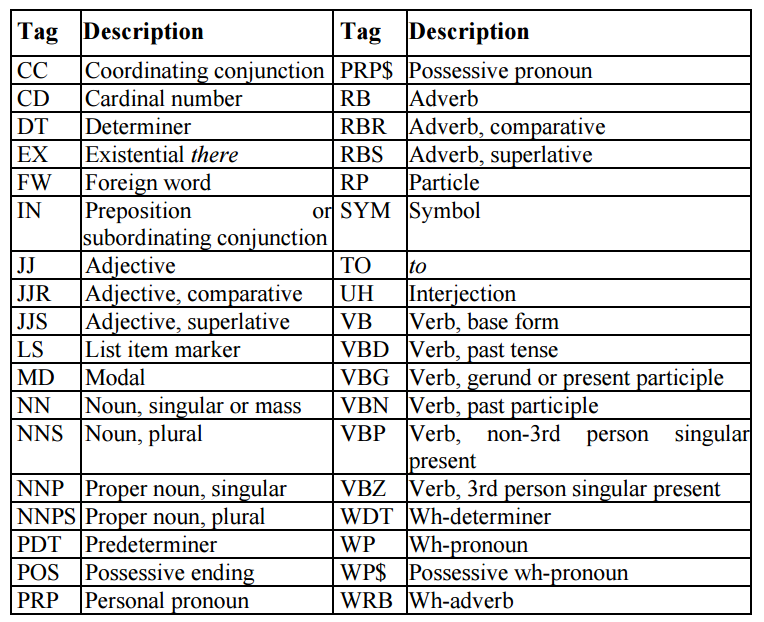
\includegraphics[width=\linewidth]{04_treebank_pos}
    \label{fig4:treebank_pos}
\end{figure}


\autoref{tab:unsupervised_example} illustrates the sentiment classification of two example tweets using a lexicon based unsupervised technique where positive and negative words are evaluated to +1 and -1 respectively. The overall score of each tweet is calculated by adding up the sentiment values of individual words.

 \subsubsection{Supervised Techniques}
 
 Supervised sentiment classification can be categorized as a natural language processing task (text classification). There are many methods to perform text classification, some of the most used classifiers are Maximum Entropy, Naive Bayes and Support Vector Machines (SVM). Before starting a sentiment classification task, the number of classes must be defined. The following are the most common approaches~\cite{liu2012sentiment}:
 
 \begin{itemize}
  \item \textbf{Two-class classifier}: Also known as polarity classification, has as an objective to classify a document as \textit{positive} or \textit{negative} which represent the two classes respectively.
  
  \item \textbf{Three-class classifier}: Similar to the two-class classifier, this one also includes subjectivity classification which means that it classifies documents as \textit{neutral} or \textit{polar} (positive or negative).
  
  \item \textbf{Multi-class classifier}: A multi-class sentiment classifier is usually based on emotional classification. Therefore, documents are classified according to emotions expressed on them (e.g. \textit{angry}, \textit{sad}, \textit{happy}, etc). 
  
\end{itemize}

\begin{table}[]
\centering
\caption{Unsupervised classification of tweets example.}
\label{tab:unsupervised_example}
\begin{tabular}{l|l}
\textbf{Tweet Content}                                                           & \textbf{Score} \\ \hline
{\color[HTML]{000000} @TylorSwift concerts are the best{\color[HTML]{036400}(+1)} :D{\color[HTML]{036400}(+1)} \#hypped{\color[HTML]{036400}(+1)}} & {\color[HTML]{036400} 3} \\ \hline
@Apple please stop selling terrible{\color[HTML]{CB0000}(-1)} music on iTunes \#mad{\color[HTML]{CB0000}(-1)}                & {\color[HTML]{CB0000}-2}                       \\ \hline
\end{tabular}
\end{table}

\pagebreak

One of the main differences between unsupervised and supervised sentiment classification methods is the training phase. Sentiment classifiers based on supervised approaches require a set of annotated documents, this annotation is usually done manually but in some cases through distant-supervision methods~\cite{go2009twitter}. Distant-supervision approach generates a training corpus by automatic means. It annotates documents based on the presence of positive or negative emojis (emoticons). The annotation accuracy of this method depends on the size of the documents, mostly used on short unit texts such as Twitter sentiment classification tasks. 

After being trained, a classifier is capable of predicting the sentiment of new input documents. The classification process requires the extraction of feature vectors from the documents; each vector contains \textit{n} numerical features. The feature sets of a classifier are essential for obtaining high accuracy. Some of the most effective features are~\cite[p. 25]{liu2012sentiment}: 

 \begin{itemize}
  \item \textbf{Terms and their frequency (bag-of-words model)}: These features are individual words (unigrams) or n-grams with associated frequency counts. N-grams are a contiguous sequence of n-tokens (words) from a given sequence of text. Besides frequency counts of the tokens, their positions might be also considered. This approach is called TF-IDF weighting scheme and is commonly used in information retrieval tasks.

    \item \textbf{Part of speech}: The part-of-speech (POS) of words in a document could be useful. For example, some research shows that adjectives are more likely to indicate sentiment than other part-of-speech words. Therefore, the number of different POS tags in a given document represents an effective feature. POS tags may also be included in other types of features such as \textit{Terms and their frequency} where unigrams are included with their respective POS tag.
    
    \item \textbf{Sentiment words and phrases}: As discussed in previews section, the presence of positive and negative words is very important for sentiment classifiers. Extracted from sentiment lexicons, the number of sentiment terms and phrases in a document represents very powerful features. 
    
    \item \textbf{Syntactic dependency}: The semantic relation between words in a document may be useful as a feature, with the usage of dependency trees is possible to find the target of a sentiment expression. However, the creation of these trees usually has a negative impact in performance times. 
    
    \item \textbf{Sentiment shifters}: These are expressions that are used to change the sentiment orientations, e.g., from positive to negative or vice versa~\cite[p. 26]{liu2012sentiment}. The most important type of sentiment shifters is negation contexts. When a negation word (e.g. \textit{not, no, never}) is present in a sentence, the sentiment score of subsequent words is inverted. For example, the sentence \textit{"the iPhone is not a good phone"} has the word \textit{good} in a negated context which translates to a negative sentiment classification of the sentence.
    
    \end{itemize}

    \begin{table}[]

    \end{table}
   

    \autoref{tab5:features_example} illustrates two example tweets with their respective vector features, these features are composed by Bag of Words model, part-of-speech tags and sentiment features. Let us explain one by one: 
    
    \begin{itemize}
        \item \textit{bag-of-words}: To reduce the sparsity of the vectors, one of the most used prepossessing steps for extracting features is the removal of stop words, which in these cases are: \textit{you, the, my, me, are}. Twitter mentions and URLs are also removed or replaced with placeholders. The resulting vectors are: 
        \begin{itemize}
            \item (1) {(@mention,1)(best,1)(<3,1)(\#happy,1)} 
            \item (2) {(bf,1)(hates,1)(:(,1)(depressed,1)}
        \end{itemize}
        Each tweet is represented on the vector space which is the union of both sets.
        
        \item \textit{part-of-speech}: This feature is composed by the count of: \textit{verbs, adjectives, nouns, adverbs}. Other POS tags could be added but these are the most relevant for sentiment classification tasks.
        
        \item \textit{sentiment}: The first tweet contains three positive tokens while the second one has three negative. As a result, the sentiment features are: (1)[3,0] \& (2)[0,3].
        
    \end{itemize}
    
    \pagebreak
    
    \subsection{SentiTrack}
    \label{sec:sentitrack}
    
    SentiTrack is a system that performs sentiment analysis of tweets in real-time using Semantic Web technologies to track stock market behaviors of a certain set of companies. In order to determine the public opinion towards a company, SentiTrack uses the Twitter API to pull tweets related to that company and process them through a sentiment analysis pipeline~\cite{danklinked}. An illustration of SentiTrack's process workflow is shown in \autoref{fig14:sentitrack_workflow}. 
    
    SentiTrack processing workflow is divided into the following three stages:
    
    \begin{enumerate}
        \item \textbf{Context Expansion}: In this stage, SentiTrack starts by selecting the set of entity companies to analyze. Then, using DBPedia and SPARQL queries a retrieval of secondary entities related to those chosen companies is performed. The secondary entities in this context are \textit{persons} and \textit{products}, e.g. \textit{Company: Microsoft, Person: Bill Gates, Product: Windows}. 
        
        \item \textbf{Stream Processing}: The set of entities obtained in previews stage are used to fed the Twitter Streaming API in order to fetch related public tweets in real-time. Then, tweets are processed for recognition and annotation of entities using DBPedia Spotlight. Moreover, those tweets with annotated entities are analyzed using a lexicon-based entity-centric sentiment classifier. The classification step intends to provide a positive, negative or neutral result based on the opinions expressed towards each of the identified entities in the tweet. Entity-centric sentiment classification approach used by SentiTrack is vary simple and not accurate enough. Therefore, an improved entity-based sentiment classifier is required for SentiTrack project.
        
        \item \textbf{Periodic Sentiment Approximation}: This stage is about analysis of the sentiment data obtained in previews steps. It creates a periodic sentiment projection in real-time about the opinions expressed in Twitter towards a target company. Additionally, a secondary system fetches real-time stock market values about the target company, this is necessary to perform a correlation evaluation with sentiment data obtained and stock values variations. 
        
    \end{enumerate}
    
    One of the contributions of this master's thesis is to integrate a more accurate sentiment classifier in SentiTrack.  
    
    \begin{figure}[H]
    \centering
    \caption[SentiTrack Workflow]{SentiTrack Workflow{~\cite{danklinked}}}
    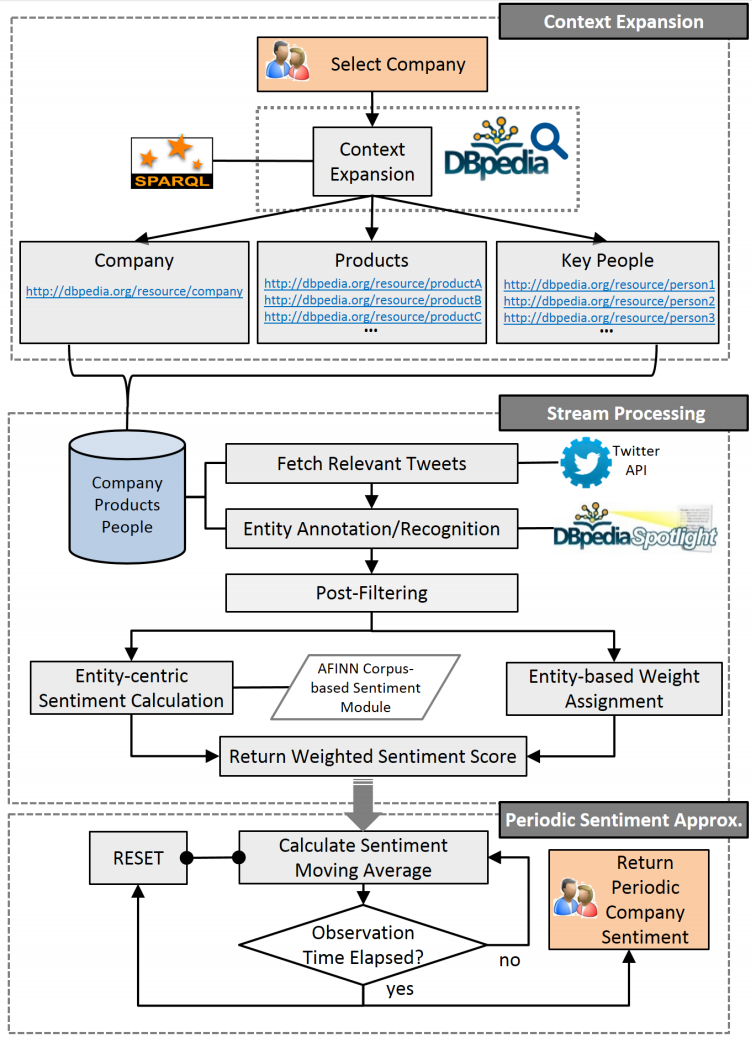
\includegraphics[width=\linewidth]{14_sentitrack_workflow}
    \label{fig14:sentitrack_workflow}
    \end{figure}
    
    \section{Named Entity Recognition}
    \label{sec:ner}
    
    Named Entity Recognition (NER) also known as named entity extraction or entity identification, is an information extraction task used mostly for natural language processing. The task consists on the extraction of structured information from unstructured text, for instance: social media networks, micro-blogging sites and e-commerce systems are constantly generating unstructured data that could be processed into valuable information for interested parties. Therefore, NER intendeds to identify elements of given input text and classify it according to a set of categories, e.g. names of persons, locations, organizations, products, values, etc ~\cite[p. 1]{nadeau2007survey}. 
    
    The most effective approaches for NER use machine learning (ML) methods to extract features of Named Entity (NE) examples classified as positive or negative, finally, these examples will form a large collection of annotated documents (training corpus).   
    
    There are three main ML techniques to perform entity identification  ~\cite[p. 4]{nadeau2007survey}:
    
    \begin{enumerate}
        \item \textit{Supervised learning}: Some of these techniques are Maximum Entropy, Decision Trees, Support Vector Machines, Conditional Random Fields and according to Nadeau ~\cite[p. 4]{nadeau2007survey}:
        \begin{displayquote}
            "A baseline Supervised learning method that is often proposed consists of tagging words of a test corpus when they are annotated as entities in the training corpus. The performance of the baseline system depends on the vocabulary transfer, which is the proportion of words, without repetitions, appearing in both training and testing corpus."
        \end{displayquote}
        Which means that NER is highly dependent on the quality of the training corpus, this will determine how accurate the classifier is.  
        
        \item \textit{Semi-supervised learning}: Semi-supervised learning (SSL) consist of a limited degree of supervision. Therefore, this technique only requires a set of seed words to start a learning process. For example, the system starts with a set of seed words related to a specific topic such as "technology". Then, the system identifies contextual clues of given words to classify new unknown terms. The accuracy this approach can achieve is not as high as fully supervised learning techniques but is effective for identification of entities related to unpopular topics where good training corpus are difficult to find. 
            
        \item \textit{Unsupervised learning}: This is a NER technique that usually depends on lexical resources (e.g., WordNet) to identify entities in a document. The types of entities are extracted from given Lexicons, therefore, the quality and number of lexical resources will define the success of this technique.
        
    \end{enumerate}
    
    
  

 
 
 
 
 

   
 
 
 
 
 
 
 